\begin{evenBlock}{HOWTO:  Shoot Hard (5 min)}

\begin{minipage}[t]{\linewidth}
    \centering
    Review these elements prior to beginning the passing drills so its fresh in their heads.

    %\begin{minipage}{.3\linewidth} % Left column and width
        %\centering
        %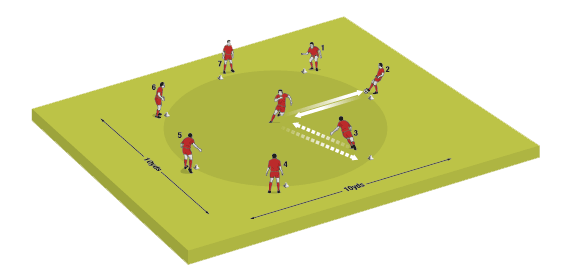
\includegraphics[width=\textwidth]{../img/Trimmed/Clocks1}
    %\end{minipage}
    %\hspace{0.05\linewidth}
    %\begin{minipage}{.6\linewidth} % Left column and width
    
        \textbf{Elements of the Power Kicking:}
    
        \begin{enumerate}
        \setlength{\itemsep}{0pt}
        \setlength{\parskip}{0pt}
        \setlength{\parsep}{0pt}
        \item Ball should be in front of the player.
        \item Non-kicking leg should be planted next to the ball with passer's toe pointed at the target.
        \item Ball should be struck with a locked ankle, the toe is pointed downward, exposing the top of the foot.  The top of the fot is the hardest part of the foot and when it strikes the ball - will impart the most energy into the ball.
        \item The kick should have a large follow through - ideally the kicker lands on his kicking foot.
        \item Landing on your kicking foot imparts all of the kickers body weight into the ball.
        \end{enumerate}
        
        \textbf{Elements of the Power Kicking:}
    
        \begin{enumerate}
        \setlength{\itemsep}{0pt}
        \setlength{\parskip}{0pt}
        \setlength{\parsep}{0pt}
        \item Ball should be in front of the player.
        \item Non-kicking leg should be planted next to the ball with passer's toe pointed at the target.
        \item Ball should be struck with a locked ankle, the toe is pointed downward, exposing the top of the foot.  The top of the fot is the hardest part of the foot and when it strikes the ball - will impart the most energy into the ball.
        \item The kick should have a large follow through - ideally the kicker lands on his kicking foot.
        \item Landing on your kicking foot imparts all of the kickers body weight into the ball.
        \end{enumerate}
    %\end{minipage}
\end{minipage}

\end{evenBlock}